\section{Introduction}

Commonly, in frequency domain studies of dynamical systems, steady-state conditions are assumed for convenience. This assumption implies that the input in the measurement window has been applied periodically for an infinitely long time, such that the system has reached steady-state with a corresponding periodic output response. There are many scenarios, however, where this assumption will be significantly violated, therefore it is important to understand the nature of the system response in the arbitrary excitation case.

For linear systems, the relationship between the measured input and output spectrum in steady-state under periodic excitation is well known, where the ratio of output to input at any given frequency is equal to the system's Frequency Response Function (FRF) at that frequency. When the system is not at steady-state, the measured output spectrum will contain an additional transient term \cite{Pintelon2012}, which is dependent on the initial conditions prior to the measurement. Modeling of a linear system's transient term was first explored in \cite{Pintelon1997} from a parametric perspective. For linear systems described nonparametrically (i.e. using an impulse response/FRF), an expression for the transient was derived in \cite{Lataire2016}. 

In order to perform a similar transient analysis for nonlinear systems, the Volterra series can be exploited as a nonparametric model structure capable of representing all time-invariant and fading memory (TIFM) nonlinear systems~\cite{Boyd1985}. For Volterra systems, steady-state frequency domain behaviour has been thoroughly explored, producing representations such as the NOFRF and GFRF models considered in this thesis. For Volterra systems under \emph{arbitrary} excitation, however, the analytic form of the transient term has yet to be determined.

In this chapter, we obtain a general expression for the measured output response of a discrete TIFM nonlinear system under arbitrary excitation. The expression is formulated in the frequency domain as a summation of steady-state and transient contributions at each nonlinear order, where the transient terms are defined analogously to the linear case \cite{Lataire2016}, providing insight into their structure and input dependencies. Moreover, the expressions can also be taken to the time domain via appropriate transformations. The validity of the derived expressions is demonstrated through numerical examples, and the implications for system identification are discussed. In particular, the possibility of extending the GPR estimation method in Chapter \ref{chap:8} to non-steady-state data is considered, where the output transients may be modeled using insights obtained in the current chapter.

\section{Preliminaries and problem formulation}

In this section, we provide rigorous definitions for the tools and transformations used in frequency domain analysis. The Volterra series and GFRF models are reiterated again, with a slightly altered formulation in the frequency domain to allow for a more convenient analysis in the sequel. For completeness, we also provide a brief summary of the linear system transient expression from \cite{Lataire2016}. 

\subsection{Frequency domain analysis}

Considering the analysis of $N$-sample signals, the following definitions are required.

\begin{defn}[$\omega_k$]
The $k$\textsuperscript{th} discrete frequency is denoted $\omega_k$ and defined as
\begin{equation}
\label{eq:DiscreteFreq}
\omega_k = \frac{2 \pi k}{N}
\end{equation}
\end{defn}

\begin{defn}[DFT]
For an $N$-sample time domain signal $\{x(t)\}_{t=0}^{N-1} \in \mathbb{R}^N$, the Discrete Fourier Transform (DFT) of $x$ at frequency bin $k$ is given by
\begin{equation}
X(k) = \sum_{t=0}^{N-1} x(t) e^{-j \omega_{k} t},
\end{equation}
where $X(k) \in \mathbb{C}$ and $\omega_{k}$ is defined in (\ref{eq:DiscreteFreq}).
\end{defn}

\begin{defn}[IDFT]
For an $N$-sample frequency domain signal $\{X(k)\}_{k=0}^{N-1} \in \mathbb{C}^N$, the inverse DFT (IDFT) of $X$ is given by
\begin{equation}
x(t) = \frac{1}{N} \sum_{k=0}^{N-1} X(k) e^{j \omega_{k} t},
\end{equation}
where $x(t) \in \mathbb{R}$.
\end{defn}

\begin{defn}[$\boldmath{m}$-DTFT]
For a discrete $m$-dimensional real function $x(\tau_1,\hdots,\tau_m)$, $\tau_1,\hdots,\tau_m \in \mathbb{N}$, and in the context of $N$-sample signals, the $N$-periodic $m$-dimensional Discrete-Time Fourier Transform ($m$-DTFT) is given by
\begin{equation}
X(k_1,\hdots,k_m) = \sum_{\tau_1=0}^{\infty} \hdots \sum_{\tau_m=0}^{\infty} x(\tau_1,\hdots,\tau_m) e^{-j \omega_{k_1} \tau_1} \hdots e^{-j \omega_{k_m} \tau_m}.
\end{equation}
\end{defn}

\begin{notation}[System input/output]
For a discrete-time dynamical system, we denote the input and output of the system as $u(t)$ and $y(t)$ respectively, where $t \in \mathbb{Z}$. If an $N$-sample portion of the input/output sequence is measured, the measured sequences are denoted $\{u(t)\}_{t=0}^{N-1}$ and $\{y(t)\}_{t=0}^{N-1}$, with corresponding $N$-point DFTs given by $\{U(k)\}_{k=0}^{N-1}$ and $\{Y(k)\}_{k=0}^{N-1}$.
\end{notation}

\subsection{Volterra series formulation}

Recall the discrete time Volterra series model structure,
\begin{equation}
\begin{aligned}
\label{eq:VolterraTD_Transients}
y(t) &= h_0 + \sum_{m=1}^{M} y_m(t), \\
y_m(t) &= \sum_{\tau_1=0}^{\infty} \hdots \sum_{\tau_m=0}^{\infty} h_m(\tau_1,\hdots,\tau_m) \prod_{\tau = \tau_1}^{\tau_m} u(t-\tau),
\end{aligned}
\end{equation}
which can be used to represent any time-invariant and fading memory nonlinear system~\cite{Boyd1985}. Note that in this chapter, we leave each Volterra kernel untruncated with infinite memory length, as this is the most general case. The maximum nonlinear order, $M$, can also be arbitrarily large.

We have also seen that the series can be expressed in the frequency domain, i.e.
\begin{equation}
Y(k) = H_0(k) + \sum_{m=1}^{M} Y_m(k),
\end{equation}
where $\{Y(k)\}_{k=0}^{N-1}$ is the DFT of $\{y(t)\}_{t=0}^{N-1}$, $Y_m(k)$ is the $m$\textsuperscript{th} order output spectrum contribution, and $H_0(k) = h_0 \delta(k)$ with $\delta(k)$ the unit impulse function. When the system is in steady-state, i.e. when $u(t)$ and $y(t)$ are $N$-periodic and $N$ samples are measured, an expression for the $m$\textsuperscript{th} order output spectrum contribution can be derived using the GFRF model structure (\ref{eqn:GFRFoutputeqn}), which for $m \geq 2$ can be written as
\begin{align}
\label{eq:VolterraFD_Transients}
Y_m^{ss}(k) = \frac{1}{N^{m-1}} \sum_{k_2=0}^{N-1} \hdots \sum_{k_m=0}^{N-1} H_m(k-k_+,k_2,\hdots,k_m) U(k-k_+) \prod_{i=2}^{m}U(k_i), 
\end{align}
where
\begin{equation}
k_+ = \sum_{i=2}^{m} k_i,
\end{equation} 
and $H_m$ is the $m$-DTFT of Volterra kernel $h_m$, typically labelled as the $m$\textsuperscript{th} order GFRF. For $m=1$, (\ref{eq:VolterraFD_Transients}) reduces to the widely known linear relation,
\begin{equation}
\label{eq:VolterraFDLin_Transients}
Y_1^{ss}(k) = H_1(k) \cdot U(k).
\end{equation} 

\subsection{Problem statement}
\label{sec:ProblemState_Transients}

The problem statement is introduced by first clarifying the system assumption.

\begin{assum}[Volterra system]
The system of interest is a causal, single-input single-output TIFM nonlinear system which satisfies the Volterra series representation (\ref{eq:VolterraTD_Transients}). 
\end{assum}

Given $N$-sample input and output measurements, $\{u(t)\}_{t=0}^{N-1}$ and $\{y(t)\}_{t=0}^{N-1}$, from the system, the aim is to find an expression for the measured frequency domain system response, $\{Y(k)\}_{k=0}^{N-1}$, as the sum of steady-state contributions, $Y_m^{ss}(k)$, and transient contributions from each nonlinear order.

\subsection{Linear system response}

The problem described in Section \ref{sec:ProblemState_Transients} has been extensively studied for the linear case, i.e. where only the $h_1(\cdot)$ kernel is non-zero in (\ref{eq:VolterraTD_Transients}). In this case, $h_1(\tau_1)$ corresponds to the system impulse response, and its DTFT, $H_1$, is the system FRF. While the steady-state contribution has been established in (\ref{eq:VolterraFDLin_Transients}), the transient contribution is less trivial. In this chapter, we consider a nonparametric approach, hence we refer to \cite{Lataire2016} for a transient expression obtained using the nonparametric impulse response model:

Consider the system input, $u(t)$, output, $y(t)$, and their $N$-sample measurements $\{u(t)\}_{t=0}^{N-1}$ and $\{y(t)\}_{t=0}^{N-1}$. We will also introduce the function $f$ as the input difference,
\begin{equation}
\label{eq:f_Transients}
f(t) =  \begin{cases} u(t) - u(t+N) & \text{for } t<0, \\ 0 & \text{for } t \geq 0, \end{cases}
\end{equation}
which is defined $\forall t$ and thus can depend on inputs $u(t)$ outside the measured window. The DFT spectrum of the measured output is now given by,
\begin{equation}
\begin{aligned}
\label{eq:LinearResponse_Transients}
Y_1(k) &= Y_1^{ss}(k) + T_1^1(k), \; \; k = 0,\hdots,N-1,\\
T_1^1(k) &= \sum_{t_1=0}^{\infty} g_1^1(t_1) e^{-j \omega_k t_1}, \\
g_1^1(t_1) &= \sum_{\tau_1=t_1+1}^{\infty} h_1(\tau_1) f(t_1-\tau_1).
\end{aligned}
\end{equation}
The linear transient contribution, $T_1^1(k)$, is formed as the DTFT of $g_1^1(t_1)$, which is a free response of the system dependent on the unmeasured initial conditions, $u(t), \; \forall t<0$. The subscript denotes the (1\textsuperscript{st}) nonlinear order of the associated system Volterra kernel, and the superscript is an index that will be required in the following sections. Note that in the case where $u(t)$ is an $N$-periodic signal applied from $t=-\infty$, then $f(t)=0 \; \forall t$, and the response reduces to the steady-state contribution as expected.

\section{The second order Volterra kernel case}

\label{sec:SecondOrderCase_Transients}

We now extend the linear result from \cite{Lataire2016}, given in (\ref{eq:LinearResponse_Transients}), to the second order Volterra kernel case, where only the kernel $h_2(\tau_1,\tau_2)$ is non-zero in (\ref{eq:VolterraTD_Transients}). First we establish some relationships between shifted time domain and DFT signals.
\begin{proposition}
\label{prop:ShiftedDFT_Transients}
For an arbitrary input, $u(t)$, and corresponding DFT signal $U(k)$ obtained via the DFT of $\{u(t)\}_{t=0}^{N-1}$, it can be easily shown that,
\begin{equation}
\label{eq:ShiftedDFT1_Transients}
\sum_{t=0}^{N-1} u(t-\tau) e^{-j \omega_{k}(t-\tau)} = U(k) + \sum_{t'=-\tau}^{-1} f(t') e^{-j \omega_{k} t'},
\end{equation}
where $f(t)$ is defined as in (\ref{eq:f_Transients}). Applying an inverse DFT, we also have that
\begin{equation}
\label{eq:ShiftedDFT2_Transients}
u(t-\tau) = \frac{1}{N} \sum_{k=0}^{N-1}\big( U(k) + \sum_{t'=-\tau}^{-1} f(t') e^{-j \omega_{k} t'} \big) e^{j \omega_{k}(t-\tau)}.
\end{equation}
\end{proposition}
%\begin{pf}
%\begin{equation}
%\begin{aligned}
%&\sum_{t=0}^{N-1} u(t-\tau) e^{-j \omega_{k} t} = e^{-j \omega_{k} \tau} \big( \sum_{t=0}^{N-1} u(t-\tau) e^{-j \omega_{k} (t-\tau)} \big) \\
%\implies &\sum_{t=0}^{N-1} u(t-\tau) e^{-j \omega_{k} (t-\tau)} \\
%&=\big( \underbrace{\sum_{t=0}^{N-1} u(t) e^{-j \omega_{k} t}}_{U(k)} + \sum_{t=-\tau}^{-1} f(t) e^{-j \omega_{k} t} \big)
%\end{aligned}
%\end{equation}
%Performing an inverse DFT on (?) yields the result in (?) \hfill \qed
%\end{pf}

The spectrum of the measured output response can now be derived for a second order Volterra kernel.

\begin{thm}
\label{thm:2ndOrderResponse_Transients}
For a system described by (\ref{eq:VolterraTD_Transients}) with only $h_2(\tau_1,\tau_2)$ non-zero, the $N$-sample measured system response can be expressed in the frequency domain as, 
\begin{equation}
\begin{aligned}
\label{eq:2ndOrderResponse_Transients}
&Y_2(k) = Y_2^{ss}(k) + 2 \; T_2^1(k) + T_2^2(k),  \; \; k = 0,\hdots,N-1,\\
&T_2^i(k) = \frac{1}{N} \sum_{k_2=0}^{N-1} \sum_{t_1=0}^{\infty} \sum_{t_2=0}^{\infty} g_2^i(t_1,t_2) e^{-j \omega_{k-k_2}t_1} e^{-j \omega_{k_2} t_2},\\
&g_2^1(t_1,t_2) = \sum_{\tau_1=t_1+1}^{\infty} \sum_{\tau_2=t_2+1-N}^{t_2} h_2(\tau_1,\tau_2) f(t_1-\tau_1) u(t_2-\tau_2),\\
&g_2^2(t_1,t_2) = \sum_{\tau_1=t_1+1}^{\infty} \sum_{\tau_2=t_2+1}^{\infty} h_2(\tau_1,\tau_2) f(t_1-\tau_1) f(t_2-\tau_2),
\end{aligned}
\end{equation}
where $Y_2(k)$ is the measured output DFT spectrum, $Y_2^{ss}(k)$ is the steady-state contribution from (\ref{eq:VolterraFD_Transients}) and $T_2^i(k)$ is the $i$\textsuperscript{th} transient contribution found from the $i$\textsuperscript{th} 2-dimensional time domain response, $g_2^i$.
\end{thm}
\begin{proof*}
From (\ref{eq:VolterraTD_Transients}), we have that
\begin{equation*}
y_2(t) = \sum_{\tau_1=0}^{\infty} \sum_{\tau_2=0}^{\infty} h_2(\tau_1,\tau_2) u(t-\tau_1) u(t-\tau_2).
\end{equation*}
Applying the DFT to each side, we obtain,
\begin{equation}
\label{eq:InitialY2_Transients}
Y_2(k) = \sum_{t=0}^{N-1} \sum_{\tau_1=0}^{\infty} \sum_{\tau_2=0}^{\infty} h_2(\tau_1,\tau_2) u(t-\tau_1) u(t-\tau_2) e^{-j \omega_k t}.
\end{equation}
The term $e^{-j \omega_k t}$ can be expressed as,
\begin{equation}
\label{eq:exponentialSplit_Transients}
e^{-j \omega_k t} =  e^{-j \omega_{k-k_2} \tau_1} e^{-j \omega_{k_2} \tau_2} e^{-j \omega_{k-k_2} (t-\tau_1)} e^{-j \omega_{k_2} (t-\tau_2)}.
\end{equation}
Substituting (\ref{eq:exponentialSplit_Transients}) into (\ref{eq:InitialY2_Transients}), we can now use the results (\ref{eq:ShiftedDFT1_Transients}) and (\ref{eq:ShiftedDFT2_Transients}) from Proposition \ref{prop:ShiftedDFT_Transients} to obtain,
\begin{equation}
\begin{aligned}
\label{eq:SecondY2_Transients}
Y_2(k) = \frac{1}{N} &\sum_{k_2=0}^{N-1} \sum_{\tau_1=0}^{\infty} \sum_{\tau_2=0}^{\infty} h_2(\tau_1,\tau_2) e^{-j \omega_{k-k_2} \tau_1} e^{-j \omega_{k_2} \tau_2} \\
&\times \Bigg( U(k-k_2) + \sum_{t_1=-\tau_1}^{-1} f(t_1) e^{-j \omega_{k-k_2} t_1}\Bigg) \Bigg( U(k_2) + \sum_{t_2=-\tau_2}^{-1} f(t_2) e^{-j \omega_{k_2} t_2}\Bigg).
\end{aligned}
\end{equation}
Expanding the 2nd line in (\ref{eq:SecondY2_Transients}), transforming the $U$ terms, applying the changes of variable, $t_i = t_i-\tau_i$, and rearranging the order of sums, it can be shown that,
\begin{equation}
\begin{aligned}
\label{eq:ThirdY2_Transients}
&Y_2(k) = \underbrace{\frac{1}{N} \sum_{k_2=0}^{N-1} \underbrace{\Bigg( \sum_{\tau_1=0}^{\infty} \sum_{\tau_2=0}^{\infty} h_2(\tau_1,\tau_2) e^{-j \omega_{k-k_2} \tau_1} e^{-j \omega_{k_2} \tau_2} \Bigg)}_{H_2(k-k_2,k_2)} U(k-k_2) U(k_2)}_{Y_2^{ss}(k)}\\
&+ \frac{1}{N} \sum_{k_2=0}^{N-1} \sum_{t_1=0}^{\infty} \sum_{t_2=0}^{\infty}\bigg( g_2^{uf}(t_1,t_2) + g_2^{fu}(t_1,t_2) + g_2^{ff}(t_1,t_2)\bigg) e^{-j \omega_{k-k_2} t_1} e^{-j \omega_{k_2} t_2},
\end{aligned}
\end{equation}
where
\begin{equation}
\begin{aligned}
&g_2^{uf}(t_1,t_2) = \sum_{\tau_1 = t_1+1-N}^{t_1} \sum_{\tau_2 = t_2+1}^{\infty} h_2(\tau_1,\tau_2) u(t_1-\tau_1) f(t_2-\tau_2),\\
&g_2^{fu}(t_1,t_2) = \sum_{\tau_1 = t_1+1}^{\infty} \sum_{\tau_2 = t_2+1-N}^{t_2} h_2(\tau_1,\tau_2) f(t_1-\tau_1) u(t_2-\tau_2) = g_2^1(t_1,t_2) ,\\
&g_2^{ff}(t_1,t_2) = \sum_{\tau_1 = t_1+1}^{\infty} \sum_{\tau_2 = t_2+1}^{\infty} h_2(\tau_1,\tau_2) f(t_1-\tau_1) f(t_2-\tau_2) = g_2^2(t_1,t_2).\\
\end{aligned}
\end{equation}
Due to the symmetry of $h_2$ and the $N$-periodicity of $e^{j \omega_k t}$, it can be shown that $g_2^{uf}$ and $g_2^{fu}$ provide equal contributions to $Y_2(k)$, hence we can replace $g_2^{uf}+g_2^{fu}$ with $2 g_2^1 = 2 g_2^{fu}$ in (\ref{eq:ThirdY2_Transients}), thus reducing it to
\begin{equation}
Y_2(k) = Y_2^{ss}(k) + 2T_2^1(k) + T_2^2(k),
\end{equation}
which completes the proof. \hfill $\qed$
\end{proof*}

From Theorem \ref{thm:2ndOrderResponse_Transients}, we see that the transient contributions from a second order Volterra kernel exhibit a considerably more complex behaviour than the linear case in (\ref{eq:LinearResponse_Transients}). The quantity $g_2^2(t_1,t_2)$ in (\ref{eq:2ndOrderResponse_Transients}) can be seen as the 2-dimensional analog to $g_1^1(t_1)$ in (\ref{eq:LinearResponse_Transients}), as it is formed from a 2D convolution of the system kernel and the difference function, $f$. The term $g_2^1(t_1,t_2)$ is also present in (\ref{eq:2ndOrderResponse_Transients}), however, which depends directly on the measured input sequence, $\{u(t)\}_{t=0}^{N-1}$.

\section{The general Volterra series case}
\label{sec:GeneralCase_Transients}

For a general TIFM nonlinear system, the intuition gained in Section \ref{sec:SecondOrderCase_Transients} can be used to formulate the contribution to the measured output spectrum from any $m$\textsuperscript{th} order kernel, $h_m$, in the corresponding Volterra series representation.
\begin{thm}
\label{thm:GeneralResponse_Transients}
For a system described by (\ref{eq:VolterraTD_Transients}), the $N$-sample measured system response can be expressed in the frequency domain as,
\begin{equation}
\begin{aligned}
\label{eq:GeneralResponse1_Transients}
&Y(k) = Y_0^{ss}(k) + \sum_{i=1}^{M} Y_m(k), \; \; k = 0,\hdots,N-1,\\
&Y_m(k) = Y_m^{ss}(k) + \sum_{i=1}^{m} \binom{m}{i} T_m^i(k),
\end{aligned}
\end{equation}
where $Y_m^{ss}(k)$ is the steady-state contribution from (\ref{eq:VolterraFD_Transients}) (and $Y_0^{ss} = H_0$), and $T_m^i$ are transient terms which emerge in the arbitrary excitation case, given by
\begin{equation}
\begin{aligned}
\label{eq:GeneralResponse2_Transients}
T_m^i(k) = &\frac{1}{N^{m-1}} \sum_{k_2=0}^{N-1} \hdots \sum_{k_{m}=0}^{N-1} \sum_{t_1=0}^{\infty} \hdots \sum_{t_m=0}^{\infty} g_m^i(t_1,\hdots,t_m) e^{-j\omega_{k-k_+}t_1} e^{-j\omega_{k_2}t_2} \hdots e^{-j\omega_{k_{m}}t_{m}},
\end{aligned}
\end{equation}
with
\begin{equation}
\begin{split}
\label{eq:GeneralResponse3_Transients}
g_m^i(t_1,\hdots,t_m) = \sum_{\tau_1=t_1+1}^{\infty} &\hdots \sum_{\tau_{i}=t_i+1}^{\infty} \sum_{\tau_{i+1}=t_{i+1}+1-N}^{t_{i+1}} \hdots \\ 
&\sum_{\tau_m=t_m+1-N}^{t_m} h_m(\tau_1,\hdots,\tau_m) \prod_{n=1}^{i}f(t_n-\tau_n)\prod_{p=i+1}^{m}u(t_p-\tau_p)
\end{split}
\end{equation}
\end{thm}
\begin{proof*}
The proof for any $m$\textsuperscript{th} order kernel follows the same steps and logic as the proof of Theorem \ref{thm:2ndOrderResponse_Transients}. \hfill $\qed$
\end{proof*}

From (\ref{eq:GeneralResponse3_Transients}), it can be seen that there are no input, $u$, terms in $g_m^m(t_1,\hdots,t_m)$, hence it can be considered as an $m$-dimensional free response (as in the linear and second order cases). All other responses, $g_m^i(t_1,\hdots,t_m)$ for $i \neq m$, depend directly on the input in the measured window. 

The mathematical structure of the response of a nonlinear system revealed in this work and given in Theorem \ref{thm:GeneralResponse_Transients} can be efficiently visualized in a `Pascal's triangle' arrangement, shown in Figure \ref{fig:NonlinearPascalTriangle}. In the figure, the $m$\textsuperscript{th} row represents the $m$\textsuperscript{th} order contribution to the total output spectrum, $Y(k)$. Furthermore, the left edge contains the steady-state contributions, while the right edge contains the free response transient terms. The remaining terms (shaded red) are all directly dependent on the measured input sequence, and only appear for $m \geq 2$.

\begin{figure}[h]
\centering
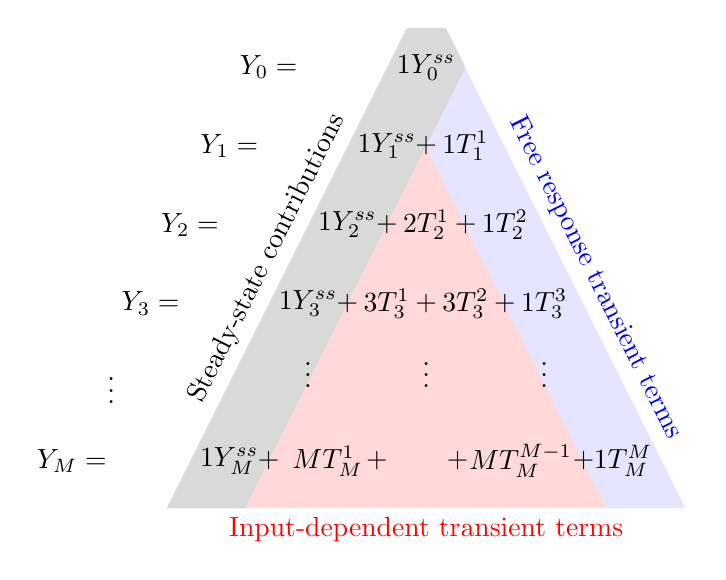
\begin{tikzpicture}[scale=1, every node/.style={scale=1}]
%\foreach \n in {0,...,4} {
%  \foreach \k in {0,...,\n} {
%	\ifthenelse{\k=0}
%    	{\node at (\k-\n/2,-\n) {${S_{\n}^{\k}}$};}
%	{\node at (\k-\n/2,-\n) {${T_{\n}^{\k}}$};}
%  }
%}

%draw shaded triangle
\fill[red!15](0,-1) -- (-2.3,-5.6) -- (2.3,-5.6)--(0,-1);
%\fill[black!15](-2.3,-5.6) -- (-3.3,-5.6) -- (-0.25,0.5)--(0.75,0.5)--(-2.3,-5.6);
\fill[black!15](-2.3,-5.6) -- (-3.3,-5.6) -- (-0.25,0.5)--(0.25,0.5)--(0.5,0)--(-2.3,-5.6);
\fill[blue!10](0,-1) -- (0.5,0) -- (3.3,-5.6) -- (2.3,-5.6)--(0,-1);

%n=0
{\node at (0,0) {${1Y_{0}^{ss}}$};}
%n=1
%{\node at (-4,-1) {(Linear term)};}
{\node at (-0.5,-1) {${1Y_{1}^{ss}}$};}
{\node at (0,-1) {${+}$};}
{\node at (0.5,-1) {${1T_{1}^{1}}$};}
%n=2
{\node at (-1,-2) {${1Y_{2}^{ss}}$};}
{\node at (-0.5,-2) {${+}$};}
{\node at (0,-2) {${2T_{2}^{1}}$};}
{\node at (0.5,-2) {${+}$};}
{\node at (1,-2) {${1T_{2}^{2}}$};}
%n=3
{\node at (-1.5,-3) {${1Y_{3}^{ss}}$};}
{\node at (-1,-3) {${+}$};}
{\node at (-0.5,-3) {${3T_{3}^{1}}$};}
{\node at (0,-3) {${+}$};}
{\node at (0.5,-3) {${3T_{3}^{2}}$};}
{\node at (1,-3) {${+}$};}
{\node at (1.5,-3) {${1T_{3}^{3}}$};}
%n=...
{\node at (-1.5,-3.8) {${\vdots}$};}
{\node at (1.5,-3.8) {${\vdots}$};}
{\node at (0,-3.8) {${\vdots}$};}
%n=M
{\node at (-2.5,-5) {${1Y_{M}^{ss}}$};}
{\node at (-2,-5) {${+}$};}
{\node at (-1.25,-5) {${MT_{M}^{1}}$};}
{\node at (-0.625,-5) {${+}$};}
{\node at (-0.1,-5) {${\hdots}$};}
{\node at (0.4,-5) {${+}$};}
{\node at (1.2,-5) {${MT_{M}^{M-1}}$};}
{\node at (2,-5) {${+}$};}
{\node at (2.5,-5)  {${1T_{M}^{M}}$};}

%Labels
\draw [very thin,white] (-3.3,-5.6) -- (-0.25,0.5) node[midway,sloped,above,xslant=0] {\textcolor{black}{Steady-state contributions}};
\draw [very thin,white] (-2.3,-5.6) -- (2.3,-5.6) node[midway,sloped,below,xslant=0] {\textcolor{red}{Input-dependent transient terms}};
\draw [very thin,white] (0.5,0) -- (3.3,-5.6) node[midway,sloped,above,xslant=0] {\textcolor{blue}{Free response transient terms}};

%Y=..
\node at (-2,0) {$Y_0 =$};
\node at (-2.5,-1) {$Y_1 =$};
\node at (-3,-2) {$Y_2 =$};
\node at (-3.5,-3) {$Y_3 =$};
\node at (-4,-4) {$\vdots$};
\node at (-4.5,-5) {$Y_M =$};

\end{tikzpicture}

\caption{A Pascal's Triangle interpretation of the frequency domain output response for a TIFM nonlinear system}
\label{fig:NonlinearPascalTriangle}
\end{figure}

\section{Numerical examples}
\label{sec:NumEx_Transients}

In this section, we will investigate the derived transient response expressions using a simple nonlinear example structure. We consider systems described by the Wiener structure shown in Figure \ref{fig:WienerStructure_Transients}, where $(\cdot)^m$ denotes exponentiation by $m$, and the discrete linear filter, $G(z)$, is chosen to be slightly underdamped with an effective memory length of approximately 60 samples, given by,
\begin{equation}
G(z) = \frac{0.75z}{z^2 -1.8z + 0.84}.
\end{equation}
The system structure is designed such that it can be represented by a single Volterra kernel, whose order we may select via our choice of $m \in \mathbb{N}$, and whose form can be obtained analytically from the impulse response of $G(z)$ (see Chapter \ref{sec:BlockStructureRelationship}).

\begin{figure}[h]
\centering
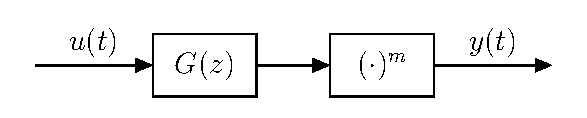
\includegraphics[scale = 0.8]{Chapter9_NonlinTransients/Wiener_Transients.pdf}
\caption{Wiener structure used for the numerical examples}
\label{fig:WienerStructure_Transients}
\end{figure}

First we examine how the (total) transient response changes with increasing nonlinear order, $m$. The total transient is defined as the difference between the measured output and the steady-state output, i.e. 
\begin{equation}
\label{eq:TotalTransient_Transients}
T_m(k) = Y_m(k) - Y_m^{ss}(k) = \sum_{i=1}^{m}\binom{m}{i} T_m^i(k),
\end{equation}
where $T_m$ is the total transient contribution from the $m$\textsuperscript{th} nonlinear order. Using the system structure in Figure \ref{fig:WienerStructure_Transients}, and setting the nonlinear exponent to $m=1, 2 \text{ and } 3$ in turn, 20 Gaussian white noise input realizations are applied to the system and the total transient is measured in a $60$-sample window. Figure \ref{fig:MC_Transients} shows the 20 transient realizations at each nonlinear order. It can be seen that the linear ($m=1$) transients are smooth functions of frequency, since they are formed purely from the free response, $g_1^1(t_1)$ in (\ref{eq:LinearResponse_Transients}). As the nonlinear order increases, however, the transients become more dominated by the white noise input in the measured window, as can be expected by observing the response structure shown in Figure \ref{fig:NonlinearPascalTriangle}.

\begin{figure}[!h]
\centering
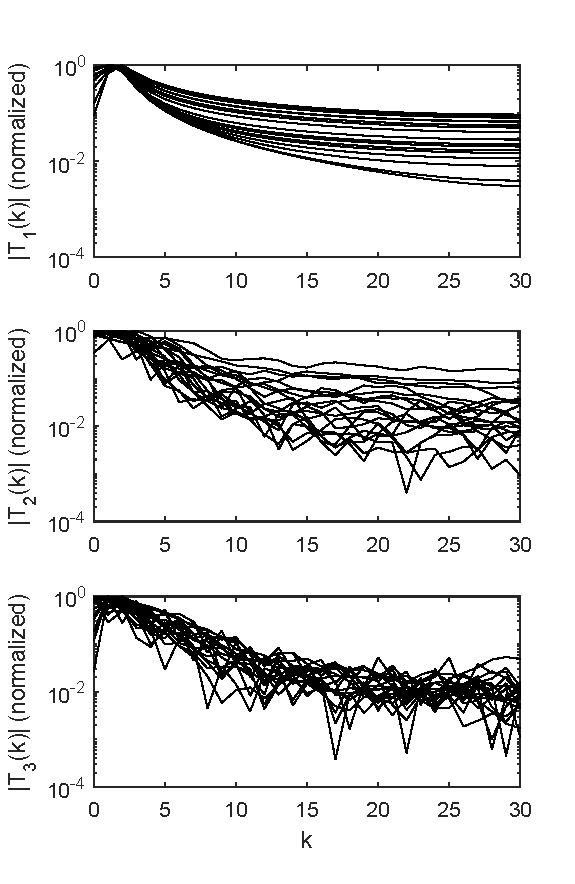
\includegraphics[width=0.6\textwidth]{Chapter9_NonlinTransients/MC_Transients3.pdf}
\caption{Total frequency domain transients for a Wiener system with linear (top), quadratic (middle) and cubic (bottom) nonlinearities}
\label{fig:MC_Transients}
\end{figure}

Next, we investigate more deeply a single realization of the system response, for the second order ($m = 2$) case. Again, using a Gaussian white noise input, we compute the two-dimensional time domain quantities, $g_2^1(t_1,t_2)$ and $g_2^2(t_1,t_2)$ from (\ref{eq:2ndOrderResponse_Transients}), which are visualized as surfaces in Figure \ref{fig:g_21+g_22}. The free response, $g_2^2(t_1,t_2)$, resembles the underlying system Volterra kernel, $h_2(\tau_1,\tau_2)$ (shown in Figure \ref{fig:h2}) while $g_2^1$ is structurally more complex.

\begin{figure}[!h]
\centering
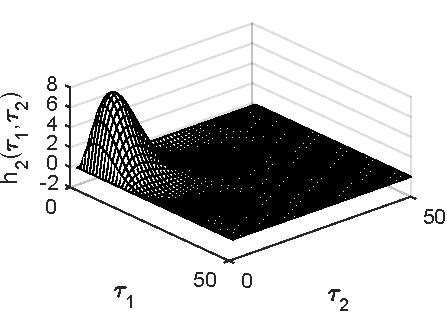
\includegraphics[width=0.5\textwidth]{Chapter9_NonlinTransients/h2_zoomedinmesh.pdf}
\caption{Volterra kernel, $h_2$, for the Wiener system with quadratic nonlinearity}
\label{fig:h2}
\end{figure}

%\begin{figure}[!tp]
%\centering
%\includegraphics[width=0.36\textwidth]{Chapter9_NonlinTransients/g_21.png}
%\caption{Time domain response, $g_2^1$, for a Wiener system with quadratic nonlinearity}
%\label{fig:g_21}
%\end{figure}
%
%\begin{figure}[t]
%\centering
%\includegraphics[width=0.36\textwidth]{Chapter9_NonlinTransients/g_22.png}
%\caption{Time domain response, $g_2^2$, for a Wiener system with quadratic nonlinearity}
%\label{fig:g_22}
%\end{figure}

\begin{figure}[!h]
\centering
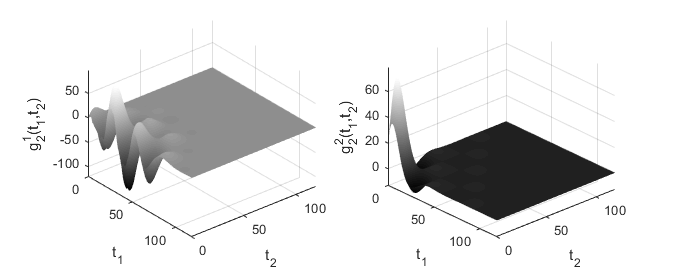
\includegraphics[width=0.95\textwidth]{Chapter9_NonlinTransients/g_2_surfaces.png}
\caption{Time domain responses $g_2^1$ (left) and $g_2^2$ (right) for a Wiener system with quadratic nonlinearity}
\label{fig:g_21+g_22}
\end{figure}

\begin{figure}[!h]
\centering
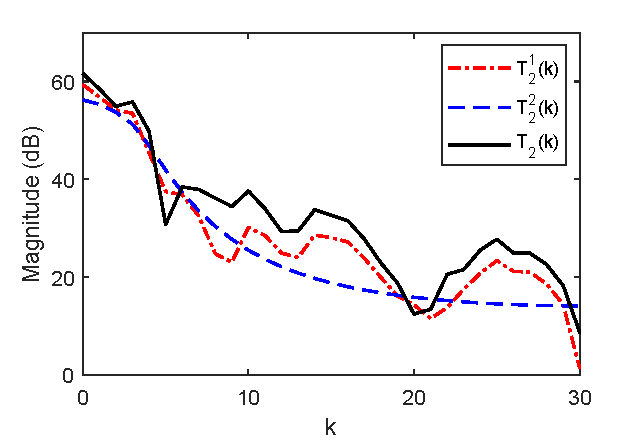
\includegraphics[width=0.65\textwidth]{Chapter9_NonlinTransients/T_2_dB.pdf}
\caption{Frequency domain transient contributions for a Wiener system with quadratic nonlinearity}
\label{fig:T_2_dB}
\end{figure}

The corresponding frequency domain transient contributions, $T_2^1(k)$ and $T_2^2(k)$, are also computed from (\ref{eq:2ndOrderResponse_Transients}), along with the total transient, $T_2(k)$ from (\ref{eq:TotalTransient_Transients}). These quantities are plotted in Figure \ref{fig:T_2_dB}. It is clear that the free response transient, $T_2^2$, has a smooth, simple structure like the linear transients, $T_1(k)$, in Figure \ref{fig:MC_Transients}. On the other hand, the input-dependent $T_2^1(k)$ has a more complex structure due to the noisy excitation signal, which is also reflected in the total transient measured from the system.

\section{Insights for system identification}

In the case where a dynamic system is identified in the frequency domain, it is not always possible or practical to enforce steady-state conditions on the system under study. As such, it is important to simultaneously identify the transient contributions present in the measured response, otherwise the quality of the estimated model will be compromised \cite{Pintelon1997}. 

For linear systems, several techniques have been developed for nonparametric estimation of the system FRF in the presence of transients. The local polynomial method (LPM) \cite{Pintelon2012}, \cite{Schoukens2009} exploits the smoothness of the transient $T_1^1(k)$ in (\ref{eq:LinearResponse_Transients}), by estimating a local polynomial around each frequency bin of the measured response in order to produce smooth estimates of the transient alongside the FRF. The local rational method (LRM) \cite{McKelvey2012} extends this idea by estimating rational transient models locally at each DFT bin. The most recent development is the Gaussian Process Regression (GPR) method designed in \cite{Lataire2016}, where the linear FRF and transient function are estimated simultaneously by exploiting the proportionality of transient and FRF covariance matrices (in a Bayesian setting) under white noise excitation. 

It is clear that in the linear case, accurate frequency domain identification relies on exploiting some special properties of the linear transient term, $T_1^1(k)$. In the case of TIFM nonlinear systems, we have shown that there are numerous contributions to a system's transient response, and many of these contributions depend heavily on the input inside the measured window. We have also seen in Section \ref{sec:NumEx_Transients} that when the input is non-smooth, the input-dependent transient contributions can be structurally complex. This observation suggests that LPM or LRM-based approaches would need significant modification in order to account for the increased complexity of transients at higher nonlinear orders. For the Bayesian frequency domain methods proposed in this part of the thesis, it is of course the linear GPR method which shows the most promise for extension.

\subsection{Transients in a parallel Hammerstein system}

In Chapter \ref{chap:7}, for the parallel Hammerstein case, the linear GPR results from \cite{Lataire2016} could be used directly in each NOFRF branch. This was because it was obvious by inspection of the model structure that the transient in any given branch is generated directly from input exponents passing through a linear filter. Now that we possess a more general framework, in Theorem \ref{thm:GeneralResponse_Transients}, for describing the system response of all TIFM nonlinear systems, it is interesting to investigate whether the derived expressions predict the linear transient behaviour of parallel Hammerstein systems. The structure of the Volterra series terms will play a key role in the analysis. 

\begin{proposition}
\label{prop:DiagonalPHkernels}
The Volterra series expansion of a system with parallel Hammerstein structure has Volterra kernels which are strictly diagonal, i.e. each kernel $h_m(\tau_1,\hdots,\tau_m)$ can only be non-zero for elements where $\tau_1 = \hdots = \tau_m$.
\end{proposition}

The result in Proposition \ref{prop:DiagonalPHkernels} is well known in the literature, with detailed discussions in \cite{Westwick2003} and \cite{Kibangou2010}. The special case of a single Hammerstein branch was also discussed in Chapter \ref{sec:BlockStructureRelationship}. In theory, the diagonal nature of the kernels can be exploited in the transient expressions of Theorem \ref{thm:GeneralResponse_Transients}, to show the reduction of all transient contributions into free responses analogous to the linear free response, $T_1^1(k)$. In practice, the analysis becomes very cumbersome as the nonlinear order, $m$, is increased, hence only the result for the second order Volterra kernel is provided.

\begin{thm}
\label{thm:FreqResponse_DiagonalKernel2}
Consider a system described by (\ref{eq:VolterraTD_Transients}) with only $h_2(\tau_1,\tau_2)$ non-zero, and where $h_2$ is a diagonal kernel. The $N$-sample measured system response can be expressed in the frequency domain as, 
\begin{align}
Y_2(k) = Y_2^{ss}(k) - T_2^2(k) + 2 T_2^{D}(k),  \; \; k = 0,\hdots,N-1,
\end{align}
where $Y_2^{ss}(k)$ is the steady-state contribution from (\ref{eq:VolterraFD_Transients}), $T_2^2(k)$ is the second order free response transient contribution in (\ref{eq:2ndOrderResponse_Transients}), and $T_2^D(k)$ is defined by
\begin{equation}
T_2^D(k) = \frac{1}{N} \sum\limits_{k_2=0}^{N-1} \sum\limits_{t_1=0}^{\infty} \sum\limits_{t_2=0}^{\infty} \sum\limits_{\tau_1=t_1+1}^{\infty} \sum\limits_{\tau_2=t_2+1}^{\infty} h_2(\tau_1,\tau_2) u(t_1-\tau_1) f(t_2-\tau_2) e^{-j \omega_{k-k_2}t_1} e^{-j \omega_{k_2} t_2} \label{eq:T2D_transients}
\end{equation}
\end{thm}

\begin{proof*}
See Appendix \ref{append:DiagonalKernelProof}. \hfill $\qed$
\end{proof*}

The result shows that for a second order \emph{diagonal} kernel there are no longer any transient contributions which depend directly on the input in the measured window, and the two remaining contributions are seen to be free responses to the initial conditions as in the linear case of $T_1^1(k)$. This provides some intuition as to why the transients in a parallel Hammerstein system behave like linear system transients. 

\subsection{GFRF estimation in the presence of transients} 

It may be possible to extend the GFRF estimation method proposed in Chapter \ref{chap:8} to simultaneously estimate transient functions in the case of arbitrary excitation. While a GPR approach will not be as simple here as in the linear case, the transient expressions derived in this chapter can still provide the insight required to design appropriate Gaussian priors for each transient contribution. For example, it can be shown that for a white noise input and Gaussian Volterra kernels, the transient response $g_m^m(t_1,\hdots,t_m)$ from (\ref{eq:GeneralResponse3_Transients}) will also be Gaussian with covariance proportional to the covariance of $h_m(\tau_1,\hdots,\tau_m)$ (as in the linear case). This result can be observed in Figures \ref{fig:h2} and \ref{fig:g_21+g_22}, where $g_2^2(t_1,t_2)$ resembles the underlying system kernel. Such a result does not exist for the input-dependent responses, $g_m^i(t_1,\hdots,t_m)$ for $i<m$, however in these cases, the covariance may be formed by combining our knowledge of the Volterra kernel covariance with the transient's known dependence on the input in the measured window. The principal challenge then is to develop a method which can construct and optimize each of the Gaussian priors for the estimation, while still maintaining accuracy and computational feasibility.

\section{Conclusion}

In this chapter, an expression was derived for the measured frequency domain system response of all fading memory nonlinear systems which can be described by the discrete Volterra series. The expression contains the steady-state response of the system at each nonlinear order, as well as a number of transient contributions which arise when the steady-state condition is not met. The different response contributions can be organized in a Pascal's triangle arrangement, revealing a highly structured view of the frequency domain response for nonlinear systems. Unlike the linear case, many of the higher order transient contributions can depend heavily on the measured input, and this may have implications for nonlinear frequency domain identification. While Hammerstein and parallel Hammerstein systems have a linear-style output transient, in general, modifications must be made to the established linear techniques if they are to be applicable in a nonlinear setting. 

\begin{subappendices}
\section{Transients proof for a second order diagonal kernel}
\label{append:DiagonalKernelProof}

\allowdisplaybreaks

The following is a proof for Theorem \ref{thm:FreqResponse_DiagonalKernel2}:

From (\ref{eq:2ndOrderResponse_Transients}) we have that
\begin{align}
&T_2^2(k) \nonumber \\
& \ \ = \frac{1}{N} \sum\limits_{k_2=0}^{N-1} \sum\limits_{t_1=0}^{\infty} \sum\limits_{t_2=0}^{\infty} \sum\limits_{\tau_1=t_1+1}^{\infty} \sum\limits_{\tau_2=t_2+1}^{\infty} h_2(\tau_1,\tau_2) f(t_1-\tau_1) f(t_2-\tau_2) e^{-j \omega_{k-k_2}t_1} e^{-j \omega_{k_2} t_2} \nonumber \\
& \ \ = \frac{1}{N} \sum\limits_{k_2=0}^{N-1} \sum\limits_{\tau_1=0}^{\infty} \sum\limits_{\tau_2=0}^{\infty} h_2(\tau_1,\tau_2) e^{-j \omega_{k-k_2}\tau_1} e^{-j \omega_{k_2} \tau_2} \sum\limits_{t_1=-\tau_1}^{-1} f(t_1) e^{-j \omega_{k-k_2}t_1}\sum\limits_{t_2=-\tau_2}^{-1} f(t_2) e^{-j \omega_{k_2} t_2}. \label{eq:PHT2}
\end{align}
The term $\sum\limits_{t_1=-\tau_1}^{-1} f(t_1) e^{-j \omega_{k-k_2}t_1}$ in (\ref{eq:PHT2}) can be expanded as follows,
\begin{align}
& \sum\limits_{t_1=-\tau_1}^{-1} f(t_1) e^{-j \omega_{k-k_2}t_1} \nonumber \\
& \ \ = \sum\limits_{t_1=-\tau_1}^{-1} (u(t_1) - u(t_1 + N)) e^{-j \omega_{k-k_2} t_1} \nonumber \\
& \ \ = \sum\limits_{t_1=-\tau_1}^{-1} u(t_1) e^{-j \omega_{k-k_2} t_1} - \sum\limits_{t_1=-\tau_1}^{-1} u(t_1 + N) e^{-j \omega_{k-k_2} t_1} \nonumber \\
& \ \ = \sum\limits_{t_1=-\tau_{1}}^{-1} u(t_1) e^{-j \omega_{k-k_2} t_1} - \sum\limits_{t_1=N-\tau_{1}}^{N-1} u(t_1) e^{-j \omega_{k-k_2} t_1} \nonumber \\
& \hspace{6.5cm} (\textrm{due to $N$-periodicity of } e^{-j \omega_{k-k_2} t_1}) \nonumber \\
& \ \ = \sum\limits_{t_1=-\tau_{1}}^{-1} u(t_1) e^{-j \omega_{k-k_2} t_1} - \sum\limits_{t_1=0}^{N-1} u(t_1) e^{-j \omega_{k-k_2} t_1} + \sum\limits_{t_1=0}^{N-\tau_1-1} u(t_1) e^{-j \omega_{k-k_2} t_1}. \label{eq:PHT6}
\end{align}
Substituting (\ref{eq:PHT6}) into (\ref{eq:PHT2}) produces the three components which make up $T_2^2(k)$:
\begin{equation}
\begin{aligned}
T_2^2(k) &= T_2^D(k) - T_2^1(k) + T_2^Q(k), \\
T_2^D(k) &= \frac{1}{N} \sum\limits_{k_2=0}^{N-1} \sum\limits_{\tau_{1}=0}^{\infty} \sum\limits_{\tau_{2}=0}^{\infty} h_{2}(\tau_{1},\tau_{2})  e^{-j \omega_{k-k_2} \tau_{1}} e^{-j \omega_{k_2} \tau_{2}}  \sum\limits_{t_1=-\tau_{1}}^{-1} u(t_1) e^{-j \omega_{k-k_2} t_1}  \\ & \hspace{0.65\textwidth}  \cdot \sum\limits_{t_2=-\tau_{2}}^{-1} f(t_2) e^{-j \omega_{k_2} t_2}, \\
T_2^Q(k) &= \frac{1}{N} \sum\limits_{k_2=0}^{N-1} \sum\limits_{\tau_{1}=0}^{\infty} \sum\limits_{\tau_{2}=0}^{\infty} h_{2}(\tau_{1},\tau_{2})  e^{-j \omega_{k-k_2} \tau_{1}} e^{-j \omega_{k_2} \tau_{2}}  \sum\limits_{t_1=0}^{N-\tau_1-1} u(t_1) e^{-j \omega_{k-k_2} t_1}  \\ & \hspace{0.65\textwidth}  \cdot \sum\limits_{t_2=-\tau_{2}}^{-1} f(t_2) e^{-j \omega_{k_2} t_2}, 
\end{aligned} 
\label{eq:PHT7}
\end{equation}
where $T_2^1(k)$ is defined in (\ref{eq:2ndOrderResponse_Transients}), and the term $T_2^D(k)$ is easily shown to be equivalent to the term in (\ref{eq:T2D_transients}). While the expression in (\ref{eq:PHT7}) holds for any second order Volterra kernel, the term $T_2^Q(k)$ can be further elaborated in the parallel Hammerstein case where $h_2(\tau_1,\tau_2)$ is a diagonal kernel. Considering only the diagonal elements $h_2(\tau,\tau)$, the following reduction is made,
\begin{equation}
\begin{aligned}
&T_2^Q(k) \\
&= \frac{1}{N} \sum\limits_{k_2=0}^{N-1} \sum\limits_{\tau=0}^{\infty} h_{2}(\tau,\tau)  e^{-j \omega_{k-k_2} \tau} e^{-j \omega_{k_2} \tau} \sum\limits_{t_1= 0}^{N-\tau-1} u(t_1) e^{-j \omega_{k-k_2} t_1} \sum\limits_{t_2= N-\tau}^{N-1} f(t_2-N) e^{-j \omega_{k_2} t_2} \\
&= \frac{1}{N} \sum\limits_{\tau=0}^{\infty} h_{2}(\tau,\tau)  e^{-j \omega_{k} \tau} \sum\limits_{t_1= 0}^{N-\tau-1} \sum\limits_{t_2= N-\tau}^{N-1} u(t_1) f(t_2-N) e^{-j \omega_{k} t_1}  \sum\limits_{k_{2}=0}^{N-1} e^{-j \omega_{k_2}(t_2 - t_1)} \\
&= 0,
\end{aligned}
\label{eq:PHT8}
\end{equation}
since (observing that $(t_2 - t_1) \in \mathbb{Z}$ and $0 < t_2 - t_1 < N$ due to the bounds of the summations),

\begin{equation*}
\begin{aligned}
\sum\limits_{k_{2}=0}^{N-1} e^{-j \omega_{k_{2}}(t_2 - t_1)} &= \sum\limits_{k_{2}=0}^{N-1} \bigg(e^{-j \frac{2 \pi (t_2 - t_1)}{N}} \bigg)^{k_{2}}  = \frac{1 - \bigg(e^{-j \frac{2 \pi (t_2 - t_1)}{N}} \bigg)^{N}}{1 - e^{-j \frac{2 \pi (t_2 - t_1)}{N}}} \\
&= \frac{1 - e^{-j 2 \pi (t_2 - t_1)}} {1 - e^{-j \frac{2 \pi (t_2 - t_1)}{N}}} = \frac{1 - 1}{1 - \underbrace{e^{-j \frac{2 \pi (t_2 - t_1)}{N}}}_{\neq 1}} = 0.
\end{aligned}
\end{equation*}
Thus (\ref{eq:PHT7}) is reduced, in the diagonal kernel case, to
\begin{equation}
T_2^1(k) = T_2^D(k) - T_2^2(k).
\label{eq:PHT9}
\end{equation}
Substituting (\ref{eq:PHT9}) into the second order response equation (\ref{eq:2ndOrderResponse_Transients}) yields
\begin{equation}
Y_2(k) = Y_2^{ss}(k) - T_2^2(k) + 2T_2^D(k)
\label{eq:PHT10}
\end{equation}
as required. \hfill $\qed$

\allowdisplaybreaks[0]

\end{subappendices}